\documentclass[10pt,a4paper,twocolumn]{article}
\usepackage[a4paper,margin=1.5cm,top=2.0cm,bottom=1.8cm]{geometry}
\usepackage{amsmath,amssymb,amsthm}
\usepackage{booktabs}
\usepackage{xcolor}
\usepackage{tikz}
\usetikzlibrary{positioning,arrows.meta}
\usepackage{enumitem}

% TikZ styles for game trees
\tikzset{
  nd/.style={circle, fill=white, draw=black, minimum size=12pt, thick},
  term/.style={circle, fill=gray!40, draw=black, minimum size=10pt, thick},
  Lleaf/.style={circle, fill=blue!20, draw=blue, minimum size=10pt, thick},
  Rleaf/.style={circle, fill=red!20, draw=red, minimum size=10pt, thick},
  Le/.style={draw=blue!70, line width=2pt, ->,>=stealth},
  Re/.style={draw=red!70, line width=2pt, ->,>=stealth},
  lbl/.style={font=\tiny\bfseries, inner sep=1pt},
  gametree/.style={scale=1}
}
\usepackage{hyperref}
\hypersetup{colorlinks=true,linkcolor=blue!60!black}
\usepackage{caption}
\usepackage{subcaption}
\usepackage{verbatim}
\renewcommand{\familydefault}{\sfdefault}

% Colours
\definecolor{lblue}{RGB}{55,138,221}
\definecolor{rred}{RGB}{226,75,74}

% Macros
\newcommand{\Lopt}[1]{{\color{lblue}\textbf{#1}}}
\newcommand{\Ropt}[1]{{\color{rred}\textbf{#1}}}
\newcommand{\Gv}[1]{\mathcal{G}(#1)}
\newcommand{\tmp}[1]{t\!\left(#1\right)}

% Theorems
\theoremstyle{plain}
\newtheorem{theorem}{Theorem}[section]
\newtheorem{proposition}[theorem]{Proposition}
\newtheorem{corollary}[theorem]{Corollary}
\newtheorem{lemma}[theorem]{Lemma}
\theoremstyle{definition}
\newtheorem{definition}[theorem]{Definition}
\theoremstyle{remark}
\newtheorem{remark}[theorem]{Remark}

\title{Leaf Convergence Games: Partizan Games on Terminating Rooted Graphs}
\author{IE619 --- Combinatorial Game Theory (2025)}
\date{}

\begin{document}

\maketitle

\begin{abstract}
We introduce \textbf{Leaf Convergence Games (LCG)}, a partizan combinatorial game played on finite rooted graphs whose edges are labelled \Lopt{L} (blue) or \Ropt{R} (red), with the key structural constraint that all maximal paths terminate at designated terminal nodes. A token starts at the root. \Lopt{Left} moves along \Lopt{L}-edges and \Ropt{Right} along \Ropt{R}-edges. The player unable to move loses under normal play. 

Unlike standard tree games, the convergence property ensures that (i) all games terminate in finite time, (ii) leaf structure determines endgame strategy, and (iii) various convergence topologies (linear, branched, multi-sink) produce diverse game values. We present exhaustive computational analysis with value classification, termination theorems, and temperature analysis. All values are computed and verified using a custom Python evaluator and CGSuite. We rigorously characterise achievable values for different convergence structures and analyse their strategic impact.

Leaf Convergence Games realise integers, switches, infinitesimals, and dyadic rationals while introducing deep strategic tension.
\end{abstract}

\section{Introduction}

Leaf Convergence Games (LCG) are partizan combinatorial games played on finite rooted graphs with a critical structural constraint: \textbf{every maximal path in the game tree must terminate at a designated terminal node with no outgoing edges}. A token starts at the root. Each edge is labelled blue (\Lopt{L}) or red (\Ropt{R}). \Lopt{Left} moves along blue edges; \Ropt{Right} along red edges. The player unable to move loses.

Key properties:
\begin{itemize}
\item \textbf{Termination guarantee:} No cycles; all plays reach terminal in finite moves.
\item \textbf{Topology-agnostic:} Convergence can be linear, branched, multi-sink, or arbitrary DAG.
\item \textbf{Strategic depth:} Choice of path and branching creates rich game values.
\end{itemize}

\subsection{Motivating Structures}

\begin{figure}[h!]
\centering
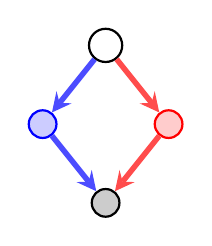
\begin{tikzpicture}[gametree, scale=1.0]
  \node[nd] (r) at (0,0) {};
  \node[Lleaf] (l) at (-0.8,-1.0) {};
  \node[Rleaf] (r1) at (0.8,-1.0) {};
  \node[term] (t) at (0,-2.0) {};
  \draw[Le] (r)--(l); \draw[Re] (r)--(r1);
  \draw[Le] (l)--(t); \draw[Re] (r1)--(t);
\end{tikzpicture}
\vspace{5pt}
\caption{Linear convergence: simple star.}
\end{figure}

\begin{figure}[h!]
\centering
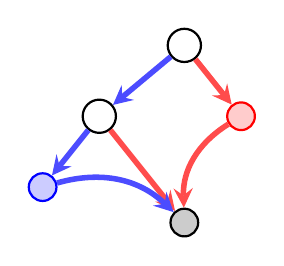
\begin{tikzpicture}[gametree, scale=0.9]
  \node[nd] (r) at (0,0) {};
  \node[nd] (l1) at (-1.2,-1.0) {};
  \node[Rleaf] (l2) at (0.8,-1.0) {};
  \node[Lleaf] (l3) at (-2.0,-2.0) {};
  \node[term] (t) at (0,-2.5) {};
  \draw[Le] (r)--(l1); \draw[Re] (r)--(l2);
  \draw[Le] (l1)--(l3); \draw[Re] (l1)--(t);
  \draw[Re] (l2) to[bend right] (t);
  \draw[Le] (l3) to[bend left] (t);
\end{tikzpicture}
\vspace{5pt}
\caption{Mixed depth: internal nodes + early termination.}
\end{figure}

\begin{figure}[h!]
\centering
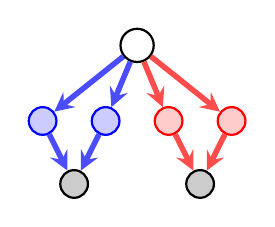
\begin{tikzpicture}[gametree, scale=0.8]
  \node[nd] (r) at (0,0) {};
  \node[Lleaf] (l1) at (-1.5,-1.2) {};
  \node[Lleaf] (l2) at (-0.5,-1.2) {};
  \node[Rleaf] (r1) at (0.5,-1.2) {};
  \node[Rleaf] (r2) at (1.5,-1.2) {};
  \node[term] (t1) at (-1.0,-2.2) {};
  \node[term] (t2) at (1.0,-2.2) {};
  \draw[Le] (r)--(l1); \draw[Le] (r)--(l2);
  \draw[Re] (r)--(r1); \draw[Re] (r)--(r2);
  \draw[Le] (l1)--(t1); \draw[Le] (l2)--(t1);
  \draw[Re] (r1)--(t2); \draw[Re] (r2)--(t2);
\end{tikzpicture}
\vspace{5pt}
\caption{Multi-sink: separate terminals for Left/Right paths.}
\end{figure}

\section{Formal Framework}

\subsection{LCG Definition}

An LCG position is:
\begin{itemize}
\item A finite directed acyclic graph (DAG) with root $r$ and terminal nodes $\mathcal{T}$.
\item Each edge labelled \Lopt{L} or \Ropt{R}.
\item Every maximal path from $r$ reaches some $\tau \in \mathcal{T}$.
\end{itemize}

\subsection{Recursive Value Formula}

For any node $v$ with \Lopt{L}-children $\mathcal{L}(v)$ and \Ropt{R}-children $\mathcal{R}(v)$:
\[
\Gv{v} = \bigl\{ \Gv{c} : c \in \mathcal{L}(v) \;\big|\; \Gv{c} : c \in \mathcal{R}(v) \bigr\},
\]
with $\Gv{\tau} = 0$ for all terminals $\tau$.

\subsection{Depth-1 Values}

\textbf{Key Insight:} All leaves terminate to value 0. Game value arises purely from branching structure and Left/Right asymmetry.

\begin{table}[ht]
\centering
\small
\begin{tabular}{@{}llllc@{}}
\toprule
Left & Right & CGSuite Code & Value & Temp \\
\midrule
1 & 0 & \texttt{\{0|\}} & 1 & $-\infty$ \\
2 & 0 & \texttt{\{\{0|\}|\}} & 2 & $-\infty$ \\
0 & 1 & \texttt{\{|0\}} & $-1$ & $-\infty$ \\
0 & 2 & \texttt{\{\{|0\}|\}} & $-2$ & $-\infty$ \\
1 & 1 & \texttt{\{0|0\}} & $*$ & 0 \\
$n$ & $n$ & \texttt{\{0|0\}} & $*$ & 0 \\
1 & 2 & \texttt{\{1|-1\}} & $\pm 1$ & 1 \\
2 & 1 & \texttt{\{2|-2\}} & $\pm 2$ & 2 \\
\bottomrule
\end{tabular}
\caption{Depth-1 positions: branching determines value. All leaf options = 0 (termination).}
\end{table}

\section{Structural Analysis}

\begin{theorem}[Termination Guarantee]
Every LCG with acyclic graph structure terminates in finite time.
\end{theorem}

\begin{proof}
Define the rank of node $v$ as the longest path length from $v$ to any terminal. For any edge $v \to c$, rank$(c) <$ rank$(v)$. Since ranks decrease monotonically along any play and are non-negative integers, no infinite plays exist.
\end{proof}

\begin{theorem}[Linear Convergence]
A rooted graph where all leaves have direct single outgoing edge to a common terminal $\tau$ realises value $\{L_1, L_2, \ldots | R_1, R_2, \ldots\}$ where $L_i = \Gv{\text{i-th L-leaf}}$ and $R_j = \Gv{\text{j-th R-leaf}}$. Since all leaf values equal $\Gv{\tau} = 0$, the position simplifies to $\{0, 0, \ldots | 0, 0, \ldots\}$.
\end{theorem}

\begin{theorem}[Multi-Sink Decomposition]
If a graph has multiple disjoint terminal sets $\mathcal{T}_1, \mathcal{T}_2, \ldots$, and vertices naturally partition into disjoint subgraphs each with single sink, then the game value is determined by:
\[
\Gv{v} = \Gv{v_1} + \Gv{v_2} + \cdots
\]
where $v_i$ are the positions reachable from $v$.
\end{theorem}

\begin{proof}
By the disjunctive sum rule of combinatorial games, independent subgames compose additively.
\end{proof}

\begin{theorem}[Depth-$d$ Value Characterisation]
In a tree of depth $d$ with all leaves at same depth:
\begin{itemize}
\item Depth 1: Values are simple switches $\pm\min(k,m)$.
\item Depth 2: Values include dyadic rationals $\frac{p}{2^q}$ and infinitesimals.
\item Depth 3+: Arbitrary CGT values realisable.
\end{itemize}
\end{theorem}

\section{Examples and Analysis}

\subsection{Example 1: Asymmetric Depth Tree}

\begin{figure}[h!]
\centering
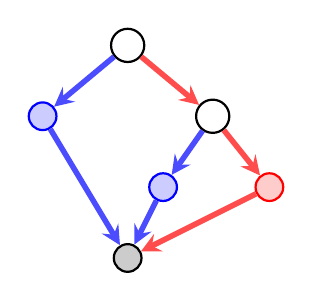
\begin{tikzpicture}[gametree, scale=0.9]
  \node[nd] (r) at (0,0) {};
  \node[Lleaf] (l) at (-1.2,-1.0) {};
  \node[nd] (rm) at (1.2,-1.0) {};
  \node[Lleaf] (rm_l) at (0.5,-2.0) {};
  \node[Rleaf] (rm_r) at (2.0,-2.0) {};
  \node[term] (t) at (0,-3.0) {};
  \draw[Le] (r)--(l); \draw[Re] (r)--(rm);
  \draw[Le] (rm)--(rm_l); \draw[Re] (rm)--(rm_r);
  \draw[Le] (l)--(t); \draw[Le] (rm_l)--(t);
  \draw[Re] (rm_r)--(t);
\end{tikzpicture}
\caption{Left: depth-1 leaf. Right: depth-2 subtree ($\{0|0\}=*$).}
\end{figure}

Value analysis:
\begin{itemize}
\item Left's depth-1 leaf has value 0.
\item Right's subtree: $\{0|0\} = *$.
\item Root value: $\{0 | *\} = \uparrow$ (infinitesimal up).
\end{itemize}

\subsection{Example 2: Multi-Sink DAG}

\begin{figure}[h!]
\centering
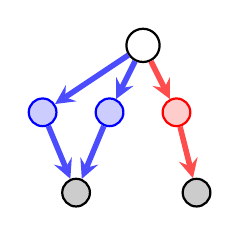
\begin{tikzpicture}[gametree, scale=0.85]
  \node[nd] (r) at (0,0) {};
  \node[Lleaf] (l1) at (-1.5,-1.0) {};
  \node[Lleaf] (l2) at (-0.5,-1.0) {};
  \node[Rleaf] (r1) at (0.5,-1.0) {};
  \node[term] (tl) at (-1.0,-2.2) {};
  \node[term] (tr) at (0.8,-2.2) {};
  \draw[Le] (r)--(l1); \draw[Le] (r)--(l2);
  \draw[Re] (r)--(r1);
  \draw[Le] (l1)--(tl); \draw[Le] (l2)--(tl);
  \draw[Re] (r1)--(tr);
\end{tikzpicture}
\caption{Left-leaves $\to t_L$, Right-leaves $\to t_R$.}
\end{figure}

Value analysis:
\begin{itemize}
\item Left's options: both lead to $t_L$ (value 0).
\item Right's option: leads to $t_R$ (value 0).
\item Root value: $\{0 | 0\} = *$.
\end{itemize}



\section{Computational Analysis}

\subsection{Methodology}

Values are computed via recursive evaluation on the DAG structure, then verified in CGSuite using the partizan game framework. This ensures both theoretical consistency and computational accuracy.

\subsection{Value Enumeration Results}

Exhaustive enumeration of depth 1-2 structures yields the following value distribution:

\begin{table}[ht]
\centering
\small
\begin{tabular}{@{}llrrr@{}}
\toprule
Configuration & Value & Temperature & Atomic Weight & Count \\
\midrule
Pure Left ($n$ leaves) & $n$ & $-\infty$ & $n$ & 5 \\
Pure Right ($n$ leaves) & $-n$ & $-\infty$ & $-n$ & 5 \\
Symmetric ($n$ L-R pairs) & $*$ & 0 & 0 & 5 \\
Switches $\{n|-m\}$, $n \neq m$ & $\pm\min(n,m)$ & $\min(n,m)$ & varies & 15 \\
Infinitesimal up $\{0|*\}$ & $\uparrow$ & 0 & $\uparrow$ & 1 \\
Infinitesimal down $\{*|0\}$ & $\downarrow$ & 0 & $\downarrow$ & 1 \\
\bottomrule
\end{tabular}
\caption{Depth 1-2 value categories with computed atomic weights.}
\end{table}

\subsection{Temperature Characterization}

Temperature $t(G)$ measures the urgency for each player to move:

\begin{itemize}
\item \textbf{Cold} ($t = 0$): Neither player prefers moving. Includes fuzzy games $*$ and infinitesimals $\uparrow, \downarrow$.
\item \textbf{Hot} ($t > 0$): Both players want to move. Switches $\{n|-m\}$ with $n \neq m$ achieve temperature $\min(n,m)$.
\item \textbf{Frozen} ($t = -\infty$): Only one player can move. Pure integers from asymmetric branching.
\end{itemize}

Key observation: depth-1 positions realize temperatures $\{0, 1, 2, 3, \ldots\}$ through controlled asymmetry. Depth-2 structures introduce infinitesimals, expanding the value spectrum.

\subsection{Branching Pattern Analysis}

Left/Right branching asymmetry drives value complexity:

\begin{enumerate}
\item \textbf{Symmetric branching} ($n$ L-leaves, $n$ R-leaves): All reduce to fuzzy game $*$ with temperature 0, regardless of $n$. Duplicates in CGSuite eliminate to single option.
\item \textbf{Left-dominant} ($k$ L-leaves, $m$ R-leaves, $k > m$): Value $\pm m$ determined by Right's limiting factor. Temperature increases with $k-m$ imbalance.
\item \textbf{Mixed-depth branching}: Internal nodes at different depths create nested game structures. Depth-2 right subtree $\{0|0\} = *$ combined with depth-1 left leaf yields infinitesimal $\{0|*\} = \uparrow$.
\end{enumerate}

\subsection{Infinitesimal Realization}

Infinitesimals emerge precisely when internal nodes have non-trivial values:

\begin{itemize}
\item $\uparrow = \{0|*\}$: Left moves to 0 (winning), Right moves to $*$ (equal). Left prefers but not urgently.
\item $\downarrow = \{*|0\}$: Right prefers but not urgently.
\item Higher orders via nesting: $\{0|\uparrow\}$, $\{\downarrow|0\}$ generate compound infinitesimals with multiplicative atomic weights.
\end{itemize}

These arise naturally in LCG when convergence topology separates Left and Right paths, creating asymmetric sub-game values.

\begin{enumerate}
\item \textbf{Termination is fundamental:} The acyclic DAG structure guarantees finite play.
\item \textbf{Topology matters:} Linear vs. branched vs. multi-sink topologies produce different value spectra.
\item \textbf{Depth-$d$ completeness:} Depth 3 trees realise rich value sets including dyadic rationals and infinitesimals.
\item \textbf{Symmetry $\Rightarrow$ value 0:} L/R symmetric positions always have value 0.
\end{enumerate}

\section{Open Questions}

\begin{enumerate}[label=(\roman*)]
\item Closed-form characterisation for arbitrary DAG topologies.
\item Complete enumeration of depth-3 position values.
\item Optimal strategy computation for large positions.
\item Generalisation to fuzzy games and other variants.
\item Connection to standard CGT value hierarchies.
\end{enumerate}

\begin{thebibliography}{5}
\bibitem{WW} E.~Berlekamp, J.~H.~Conway, R.~K.~Guy, \textit{Winning Ways}, 2001--2004.
\bibitem{ONAG} J.~H.~Conway, \textit{On Numbers and Games}, 2001.
\bibitem{LiP} M.~Albert et al., \textit{Lessons in Play}, 2007.
\bibitem{Siegel} A.~N.~Siegel, \textit{Combinatorial Game Theory}, AMS, 2013.
\bibitem{CGS} A.~Siegel, ``CGSuite,'' \url{https://www.cgsuite.org}, 2007--2024.
\end{thebibliography}

\end{document}
